% System design of the MonetaryPolicyTransmission live forecasting experiment.
% Build: cd docs/slides && latexmk -pdf system_design.tex  (or pdflatex twice)
\documentclass[aspectratio=169,10pt]{beamer}

\usetheme{default}
\usecolortheme{default}
\setbeamertemplate{navigation symbols}{}
\setbeamertemplate{footline}[frame number]

\usepackage[T1]{fontenc}
\usepackage{lmodern}
\usepackage{booktabs}
\usepackage{amsmath}
\usepackage{tikz}
\usetikzlibrary{arrows.meta,positioning,fit,calc,shapes.geometric,decorations.pathreplacing}

% Palette
\definecolor{ecbblue}{HTML}{003299}
\definecolor{bank}{HTML}{1F6FB2}
\definecolor{hh}{HTML}{C0611B}
\definecolor{ok}{HTML}{2E7D32}
\definecolor{warn}{HTML}{B71C1C}
\definecolor{soft}{HTML}{EEF2F8}
\definecolor{grey}{HTML}{6B7280}

\setbeamercolor{frametitle}{fg=ecbblue}
\setbeamercolor{title}{fg=ecbblue}
\setbeamercolor{structure}{fg=ecbblue}
\setbeamerfont{frametitle}{series=\bfseries}

\tikzset{
  box/.style={draw=ecbblue!70, fill=soft, rounded corners=3pt, align=center,
              inner sep=4pt, minimum height=9mm, font=\footnotesize},
  flow/.style={-{Stealth[length=2.2mm]}, thick, ecbblue!80},
  tag/.style={font=\scriptsize\itshape, text=grey},
}

\title{LLM Agents Forecasting Euro Area\\Monetary Policy Transmission}
\subtitle{System design of a pre-registered live forecasting experiment\\Round 1: \texttt{ea-2026q3-live}}
\date{October 2026}

\begin{document}

% ------------------------------------------------------------------
\begin{frame}
  \titlepage
\end{frame}

% ------------------------------------------------------------------
\begin{frame}{The idea in one slide}
  \begin{columns}[T]
    \begin{column}{0.52\textwidth}
      \textbf{Question.} Can LLM agents that role-play euro area \textcolor{bank}{\textbf{banks}} and
      \textcolor{hh}{\textbf{households}} forecast how the real survey respondents reacted to the 2026
      tightening --- \emph{before} the surveys are published?

      \vspace{2mm}
      \textbf{Why live?} Back-testing on past surveys is contaminated: the answers may sit in the
      training data. Forecasting an \emph{unreleased} number is the only clean test.

      \vspace{2mm}
      \textbf{Second question.} Does any skill come from \emph{reasoning} or from \emph{memorised} data?
      A panel of models released before and after the shock answers this.
    \end{column}
    \begin{column}{0.45\textwidth}
      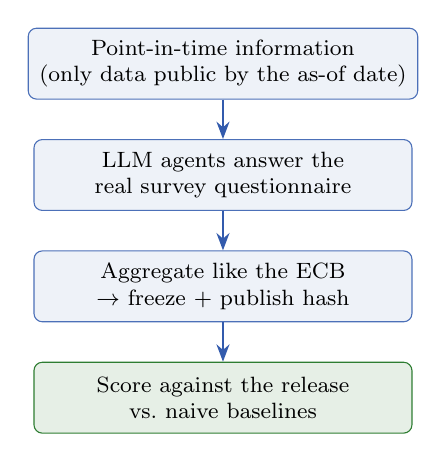
\begin{tikzpicture}[node distance=5mm]
        \node[box, minimum width=48mm] (a) {Point-in-time information\\(only data public by the as-of date)};
        \node[box, below=of a, minimum width=48mm] (b) {LLM agents answer the\\real survey questionnaire};
        \node[box, below=of b, minimum width=48mm] (c) {Aggregate like the ECB\\$\rightarrow$ freeze + publish hash};
        \node[box, below=of c, minimum width=48mm, fill=ok!12, draw=ok] (d) {Score against the release\\vs.\ naive baselines};
        \draw[flow] (a) -- (b); \draw[flow] (b) -- (c); \draw[flow] (c) -- (d);
      \end{tikzpicture}
    \end{column}
  \end{columns}
\end{frame}

% ------------------------------------------------------------------
\begin{frame}{Timeline: shock, knowledge gradient, forecast window}
  \centering
  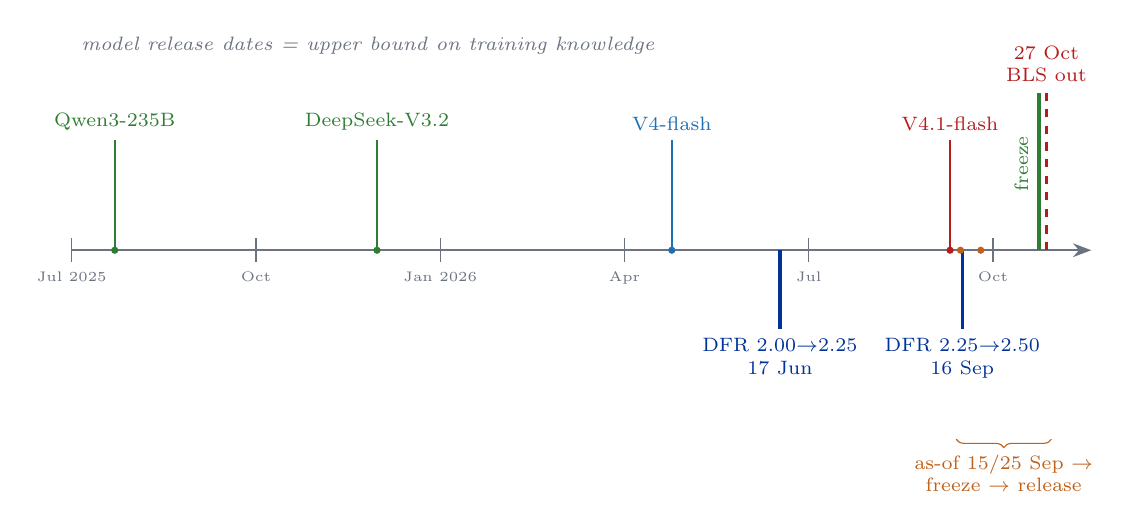
\begin{tikzpicture}[x=7.8mm, y=1mm]
    % axis: months from Jul 2025 (0) to Nov 2026 (16)
    \draw[thick, grey, -{Stealth}] (0,0) -- (16.6,0);
    \foreach \m/\l in {0/Jul 2025, 3/Oct, 6/Jan 2026, 9/Apr, 12/Jul, 15/Oct}
      { \draw[grey] (\m,-1.5) -- (\m,1.5); \node[font=\tiny, grey, below] at (\m,-1.5) {\l}; }

    % model releases (above)
    \foreach \x/\n/\c in {0.7/Qwen3-235B/ok, 4.97/DeepSeek-V3.2/ok, 9.77/V4-flash/bank, 14.3/V4.1-flash/warn}
      { \fill[\c] (\x,0) circle (1.3pt);
        \draw[\c, thick] (\x,0) -- (\x,14);
        \node[font=\scriptsize, text=\c, above, align=center] at (\x,14) {\n}; }
    \node[tag, anchor=west] at (0,26) {model release dates = upper bound on training knowledge};

    % policy events (below)
    \foreach \x/\n in {11.53/{DFR 2.00$\to$2.25\\17 Jun}, 14.5/{DFR 2.25$\to$2.50\\16 Sep}}
      { \draw[ecbblue, very thick] (\x,0) -- (\x,-10);
        \node[font=\scriptsize, text=ecbblue, below, align=center] at (\x,-10) {\n}; }

    % as-of dates, freeze and release
    \foreach \x in {14.47, 14.8} \fill[hh] (\x,0) circle (1.3pt);
    \draw[decorate, decoration={brace, amplitude=3pt, mirror}, hh] (14.4,-24) -- (15.95,-24)
      node[midway, below=2pt, font=\scriptsize, text=hh, align=center] {as-of 15/25 Sep $\to$\\freeze $\to$ release};
    \draw[ok, very thick] (15.75,0) -- (15.75,20) node[pos=0.55, rotate=90, above, font=\scriptsize, text=ok] {freeze};
    \draw[warn, very thick, dashed] (15.87,0) -- (15.87,20) node[above, font=\scriptsize, text=warn, align=center] {27 Oct\\BLS out};
  \end{tikzpicture}

  \vspace{1mm}
  \footnotesize
  Arms: \textcolor{ok}{\textbf{clean}} (pre-shock) \quad
  \textcolor{bank}{\textbf{pre-hike}} \quad
  \textcolor{warn}{\textbf{post-hike}} (contamination risk). \;
  Freeze before 26 Oct; the CES September wave follows in late October.
\end{frame}

% ------------------------------------------------------------------
\begin{frame}{System architecture}
  \centering
  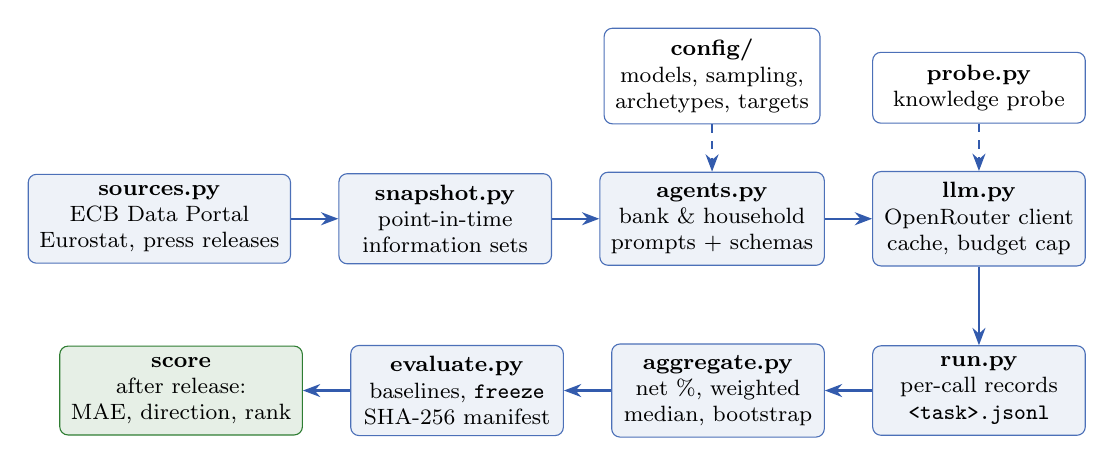
\begin{tikzpicture}[node distance=4mm and 6mm]
    \node[box, minimum width=27mm] (src) {\textbf{sources.py}\\ECB Data Portal\\Eurostat, press releases};
    \node[box, right=of src, minimum width=27mm] (snap) {\textbf{snapshot.py}\\point-in-time\\information sets};
    \node[box, right=of snap, minimum width=27mm] (ag) {\textbf{agents.py}\\bank \& household\\prompts + schemas};
    \node[box, right=of ag, minimum width=27mm] (llm) {\textbf{llm.py}\\OpenRouter client\\cache, budget cap};

    \node[box, below=10mm of llm, minimum width=27mm] (run) {\textbf{run.py}\\per-call records\\\texttt{<task>.jsonl}};
    \node[box, left=of run, minimum width=27mm] (agg) {\textbf{aggregate.py}\\net \%, weighted\\median, bootstrap};
    \node[box, left=of agg, minimum width=27mm] (frz) {\textbf{evaluate.py}\\baselines, \texttt{freeze}\\SHA-256 manifest};
    \node[box, left=of frz, minimum width=27mm, fill=ok!12, draw=ok] (sc) {\textbf{score}\\after release:\\MAE, direction, rank};

    \node[box, above=6mm of ag, minimum width=27mm, fill=white] (cfg) {\textbf{config/}\\models, sampling,\\archetypes, targets};
    \node[box, above=6mm of llm, minimum width=27mm, fill=white] (pr) {\textbf{probe.py}\\knowledge probe};

    \draw[flow] (src) -- (snap); \draw[flow] (snap) -- (ag); \draw[flow] (ag) -- (llm);
    \draw[flow] (llm) -- (run); \draw[flow] (run) -- (agg); \draw[flow] (agg) -- (frz); \draw[flow] (frz) -- (sc);
    \draw[flow, dashed] (cfg) -- (ag); \draw[flow, dashed] (pr) -- (llm);
  \end{tikzpicture}

  \vspace{3mm}
  \footnotesize
  One CLI: \texttt{data} $\rightarrow$ \texttt{estimate} $\rightarrow$ \texttt{run -{}-tasks probe} $\rightarrow$
  \texttt{run -{}-tasks bls ces} $\rightarrow$ \texttt{baselines} $\rightarrow$ \texttt{freeze} $\rightarrow$ \texttt{score}
\end{frame}

% ------------------------------------------------------------------
\begin{frame}{Point-in-time information sets}
  Agents see only data whose \emph{conservative} publication date is on or before the as-of date ---
  and no narrative written by the researchers.

  \vspace{3mm}
  \footnotesize
  \begin{tabular}{@{}llp{82mm}@{}}
    \toprule
    Task & As of & Contents \\
    \midrule
    \textcolor{hh}{CES households} & 15 Sep 2026 & own-country HICP; first paragraph of the 10 Sep ECB press release;
      own-country mortgage rate (mortgagors only) \\
    \textcolor{bank}{BLS banks} & 25 Sep 2026 & DFR history, \texteuro STR, 12m Euribor, HICP (EA, DE, FR, IT, ES),
      MFI lending rates, previous BLS rounds, full 10 Sep press release \\
    \bottomrule
  \end{tabular}

  \vspace{4mm}
  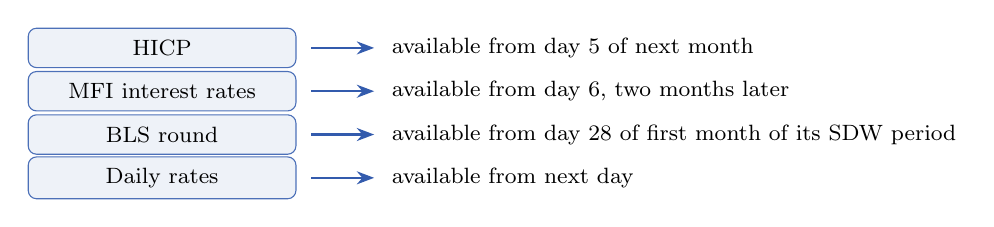
\begin{tikzpicture}
    \foreach \y/\s/\r in {0/HICP/{day 5 of next month},
                          -0.55/MFI interest rates/{day 6, two months later},
                          -1.1/BLS round/{day 28 of first month of its SDW period},
                          -1.65/Daily rates/{next day}}
      { \node[box, minimum width=34mm, minimum height=5mm, anchor=west] at (0,\y) {\s};
        \draw[flow] (3.6,\y) -- (4.4,\y);
        \node[font=\footnotesize, anchor=west] at (4.5,\y) {available from \r}; }
  \end{tikzpicture}
\end{frame}

% ------------------------------------------------------------------
\begin{frame}{Knowledge probe: does a model already know the 2026 hikes?}
  \begin{columns}[T]
    \begin{column}{0.40\textwidth}
      \footnotesize
      Six DFR questions, 3 samples each (1 at $T{=}0$, 2 at $T{=}1$):
      \begin{itemize}
        \item \textbf{control} (2024, 2025): can the model answer at all?
        \item \textbf{boundary} (1 Jan 2026): answerable by assuming no change
        \item \textbf{target} (Jun, Sep 2026, first hike): only if trained on post-shock data
      \end{itemize}
      Flag ``knows 2026'' = any target correct. Diagnostic only; nobody is excluded.
    \end{column}
    \begin{column}{0.58\textwidth}
      \scriptsize
      \textbf{Round 1 result} (correct answers out of 3)\\[1mm]
      \begin{tabular}{@{}lcccc@{}}
        \toprule
        & Qwen3 & DS-V3.2 & V4-flash & V4.1-flash \\
        \midrule
        2024-06 control (3.75) & 2 & 3 & 3 & 3 \\
        2025-06 control (2.00) & 0 & 0 & 0 & 2 \\
        2026-01 boundary (2.00) & 0 & 0 & 0 & 1 \\
        \midrule
        2026-06 target (2.25) & \textcolor{ok}{0} & \textcolor{ok}{0} & \textcolor{ok}{0} & \textcolor{ok}{0} \\
        2026-09 target (2.50) & \textcolor{ok}{0} & \textcolor{ok}{0} & \textcolor{ok}{0} & \textcolor{ok}{0} \\
        First hike (2.25) & \textcolor{ok}{0} & \textcolor{ok}{0} & \textcolor{ok}{0} & \textcolor{ok}{0} \\
        \bottomrule
      \end{tabular}

      \vspace{2mm}
      No model knows the 2026 hikes. Knowledge fades through 2025 even for the
      September 2026 model.
    \end{column}
  \end{columns}
\end{frame}

% ------------------------------------------------------------------
\begin{frame}{Bank agents: nine archetypes answer the BLS questionnaire}
  \begin{columns}[T]
    \begin{column}{0.47\textwidth}
      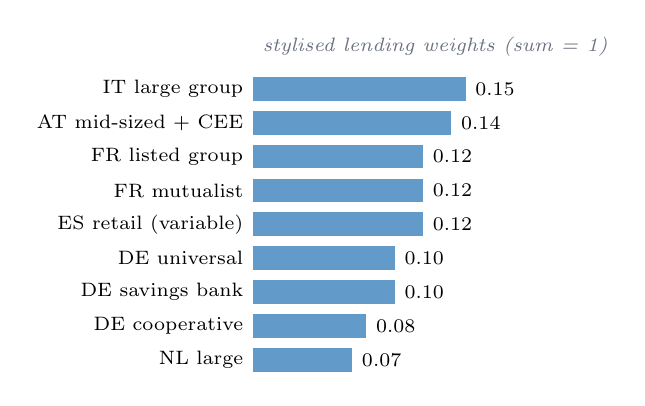
\begin{tikzpicture}[x=40mm, y=4.3mm]
        \foreach \i/\n/\w in {0/IT large group/0.15, 1/AT mid-sized + CEE/0.14, 2/FR listed group/0.12,
                              3/FR mutualist/0.12, 4/ES retail (variable)/0.12, 5/DE universal/0.10,
                              6/DE savings bank/0.10, 7/DE cooperative/0.08, 8/NL large/0.07}
          { \fill[bank!70] (0,-\i) rectangle (\w*4.5,-\i-0.7);
            \node[font=\scriptsize, anchor=east] at (0,-\i-0.35) {\n};
            \node[font=\scriptsize, anchor=west] at (\w*4.5,-\i-0.35) {\w}; }
        \node[tag, anchor=west] at (0,0.9) {stylised lending weights (sum = 1)};
      \end{tikzpicture}
    \end{column}
    \begin{column}{0.51\textwidth}
      \footnotesize
      \textbf{Prompt} \; system: \emph{``You are the senior loan officer \ldots{} Today's date is
      2026-09-25; you know nothing that happened after it.''}\\
      user: data block + ECB press release + six questions.

      \vspace{2mm}
      \textbf{Questions} \; credit standards for
      \{enterprises, housing, consumer credit\} $\times$ \{past 3m, next 3m\}

      \vspace{2mm}
      \textbf{Answer scale} (ECB coding)\\[1mm]
      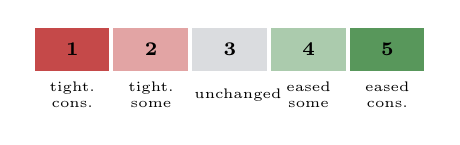
\begin{tikzpicture}[x=10mm]
        \foreach \k/\c/\l in {1/warn!80/tight. cons., 2/warn!40/tight. some, 3/grey!25/unchanged,
                              4/ok!40/eased some, 5/ok!80/eased cons.}
          { \fill[\c] (\k-1,0) rectangle (\k-0.05,0.55);
            \node[font=\scriptsize\bfseries] at (\k-0.52,0.27) {\k};
            \node[font=\tiny, align=center, text width=9mm] at (\k-0.52,-0.3) {\l}; }
      \end{tikzpicture}

      \vspace{1mm}
      Structured JSON output with a \texttt{main\_factors} rationale.\\
      30 samples per archetype per model at $T{=}1$.
    \end{column}
  \end{columns}
\end{frame}

% ------------------------------------------------------------------
\begin{frame}{Household agents: 60 personas, two information arms}
  \begin{columns}[T]
    \begin{column}{0.47\textwidth}
      \centering
      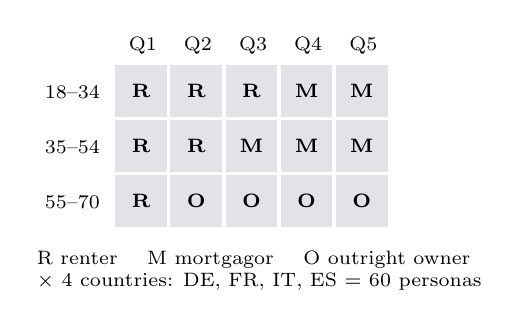
\begin{tikzpicture}[x=7mm, y=7mm]
        \foreach \r/\a in {0/18--34, 1/35--54, 2/55--70}
          \node[font=\scriptsize, anchor=east] at (-0.1,-\r-0.5) {\a};
        \foreach \q in {1,...,5} \node[font=\scriptsize] at (\q-0.5,0.35) {Q\q};
        % tenure grid: R renter, M mortgagor, O outright owner
        \foreach \r/\row in {0/{R,R,R,M,M}, 1/{R,R,M,M,M}, 2/{R,O,O,O,O}} {
          \foreach \t [count=\q] in \row {
            \ifx\t M \def\col{hh!70}\else\ifx\t O \def\col{hh!35}\else\def\col{grey!20}\fi\fi
            \fill[\col] (\q-1,-\r) rectangle (\q-0.06,-\r-0.94);
            \node[font=\scriptsize\bfseries] at (\q-0.53,-\r-0.47) {\t};
          }
        }
        \node[font=\scriptsize, align=left, anchor=north west] at (-1.6,-3.2)
          {R renter \quad M mortgagor \quad O outright owner\\
           $\times$ 4 countries: DE, FR, IT, ES = 60 personas};
      \end{tikzpicture}
    \end{column}
    \begin{column}{0.51\textwidth}
      \footnotesize
      \textbf{Persona} = age band (weights .27/.38/.35) $\times$ income quintile (equal);
      mortgagors hold the country's dominant mortgage type (ES variable, DE/FR fixed, \ldots).

      \vspace{2mm}
      \textbf{Two arms}
      \begin{itemize}
        \item \textcolor{hh}{\texttt{news}} (primary): own-country HICP, the ECB announcement,
              own mortgage rate --- facts a household could have seen.
        \item \texttt{minimal}: persona and date only. A model that still produces 2026-level
              answers here betrays memorised data.
      \end{itemize}

      \textbf{Output}: perceived past and expected next-12-month inflation (\%).
      8 samples per persona $\times$ arm $\times$ model.
    \end{column}
  \end{columns}
\end{frame}

% ------------------------------------------------------------------
\begin{frame}{Aggregation: from agent answers to survey statistics}
  \begin{columns}[T]
    \begin{column}{0.5\textwidth}
      \textcolor{bank}{\textbf{BLS net percentage}}
      \[
        \text{Net}_q = 100 \sum_{b} w_b \,\Big(\underbrace{\mathrm{Pr}_b[1\text{--}2]}_{\text{tightened}}
                       - \underbrace{\mathrm{Pr}_b[4\text{--}5]}_{\text{eased}}\Big)
      \]
      for each of the 6 questions $q$; shares are over bank $b$'s 30 samples.
      Positive = net tightening, as in the ECB release.
    \end{column}
    \begin{column}{0.48\textwidth}
      \textcolor{hh}{\textbf{CES country median}}
      \[
        \text{Med}_c = \operatorname{wmedian}\big\{x_{p,s}\,;\; \tfrac{w_p}{n_p}\big\}_{p\in c}
      \]
      weighted median of \texttt{expected\_inflation\_next\_12m} over all persona samples in
      country $c$. Answers with $|x|>100$ are dropped and counted.
    \end{column}
  \end{columns}

  \vspace{5mm}
  \begin{block}{Uncertainty and failures}
    \footnotesize
    90\% intervals from 1{,}000 bootstrap draws resampling answers \emph{within} each bank / persona.
    Failed calls (API or JSON errors) are counted and reported, never imputed.
  \end{block}
\end{frame}

% ------------------------------------------------------------------
\begin{frame}{Targets, baselines and hypotheses}
  \footnotesize
  \begin{columns}[T]
    \begin{column}{0.48\textwidth}
      \textbf{Targets} (ECB Data Portal)\\[1mm]
      \scriptsize
      \begin{tabular}{@{}lll@{}}
        \toprule
        Survey & Statistic & Release \\
        \midrule
        \textcolor{bank}{BLS} & 3 items $\times$ past/next 3m & 27 Oct 2026 \\
        \textcolor{hh}{CES} & median 12m exp., DE/FR/IT/ES & late Oct 2026 \\
        \bottomrule
      \end{tabular}
      \footnotesize

      \vspace{3mm}
      \textbf{Baselines} (fetched before freezing)
      \begin{itemize}
        \item BLS persistence: previous round's value
        \item BLS banks' own previous expectation (past-3m targets)
        \item CES persistence: August 2026 value
      \end{itemize}
    \end{column}
    \begin{column}{0.5\textwidth}
      \textbf{Hypotheses}
      \begin{description}[H3]
        \item[H1] Bank agents beat both BLS baselines on MAE.
        \item[H2] Household agents (\texttt{news}) beat CES persistence on MAE and rank the four
                  countries correctly.
        \item[H3] Skill does \emph{not} rise with model release date; pre-shock models give no
                  2026-level answers in the \texttt{minimal} arm.
      \end{description}

      \textbf{Metrics}: MAE (pp), direction hits vs.\ previous value, Spearman rank (CES).
      Persistence is a strong baseline --- a null result is reported the same way.
    \end{column}
  \end{columns}
\end{frame}

% ------------------------------------------------------------------
\begin{frame}{Integrity safeguards}
  \centering
  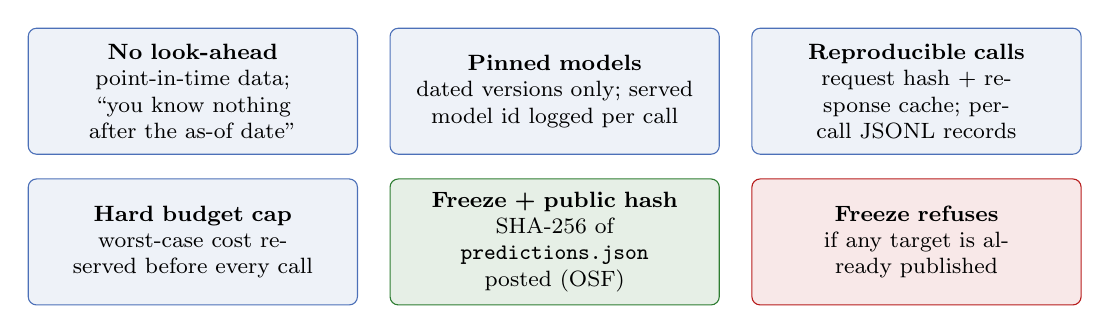
\begin{tikzpicture}[node distance=3mm and 4mm]
    \node[box, text width=39mm, minimum height=16mm] (a) {\textbf{No look-ahead}\\point-in-time data;
      ``you know nothing after the as-of date''};
    \node[box, right=of a, text width=39mm, minimum height=16mm] (b) {\textbf{Pinned models}\\dated versions only;
      served model id logged per call};
    \node[box, right=of b, text width=39mm, minimum height=16mm] (c) {\textbf{Reproducible calls}\\request hash + response
      cache; per-call JSONL records};
    \node[box, below=of a, text width=39mm, minimum height=16mm] (d) {\textbf{Hard budget cap}\\worst-case cost reserved
      before every call};
    \node[box, below=of b, text width=39mm, minimum height=16mm, fill=ok!12, draw=ok] (e) {\textbf{Freeze + public hash}\\SHA-256 of
      \texttt{predictions.json} posted (OSF)};
    \node[box, below=of c, text width=39mm, minimum height=16mm, fill=warn!10, draw=warn] (f) {\textbf{Freeze refuses}\\if any target
      is already published};
  \end{tikzpicture}

  \vspace{4mm}
  \footnotesize
  Pre-registered design; every post-freeze change is logged under \emph{Deviations}.
\end{frame}

% ------------------------------------------------------------------
\begin{frame}{Scale of round 1}
  \centering
  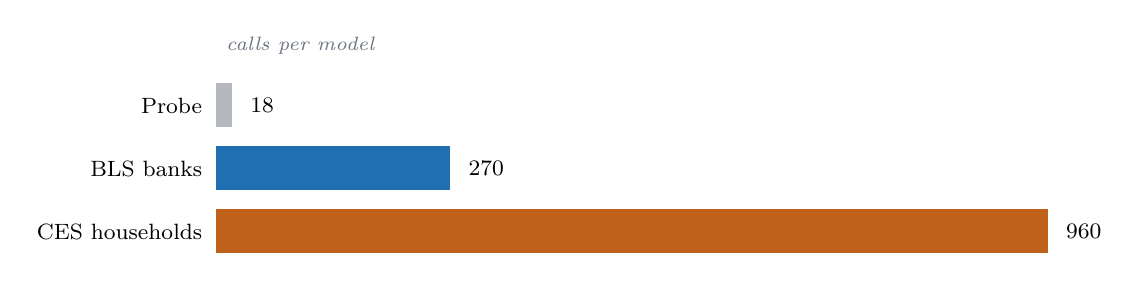
\begin{tikzpicture}[x=0.11mm, y=8mm]
    \foreach \i/\n/\v/\c in {0/Probe/18/grey!50, 1/BLS banks/270/bank, 2/CES households/960/hh}
      { \fill[\c] (0,-\i) rectangle (\v,-\i-0.7);
        \node[font=\footnotesize, anchor=east] at (-5,-\i-0.35) {\n};
        \node[font=\footnotesize, anchor=west] at (\v+10,-\i-0.35) {\v}; }
    \node[tag, anchor=west] at (0,0.6) {calls per model};
  \end{tikzpicture}

  \vspace{4mm}
  \footnotesize
  \begin{tabular}{@{}lr@{}}
    BLS: 9 archetypes $\times$ 30 samples & 270 \\
    CES: 60 personas $\times$ 2 arms $\times$ 8 samples & 960 \\
    \midrule
    $\times$ 4 models $\Rightarrow$ forecast calls & 4{,}920 \\
    Worst-case cost (budget cap \$10 per CLI call) & \$8.40 \\
  \end{tabular}
\end{frame}

% ------------------------------------------------------------------
\begin{frame}{Roadmap}
  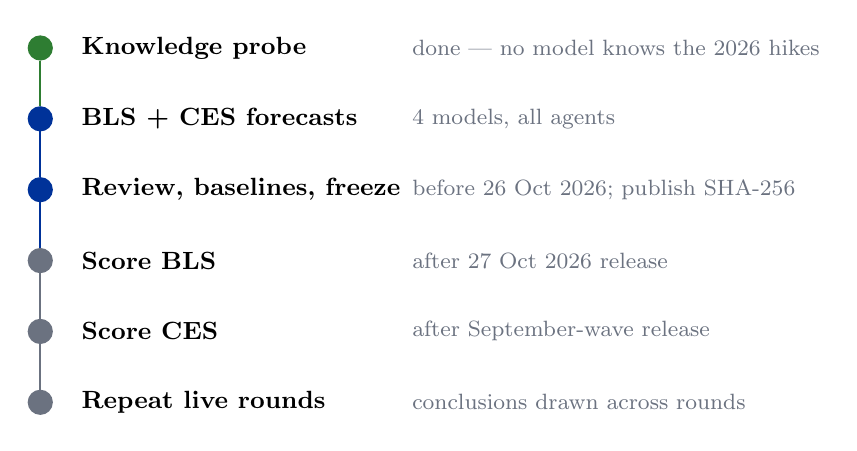
\begin{tikzpicture}[node distance=3mm]
    \foreach \i/\t/\d/\c in {0/Knowledge probe/done --- no model knows the 2026 hikes/ok,
                             1/BLS + CES forecasts/{4 models, all agents}/ecbblue,
                             2/{Review, baselines, freeze}/{before 26 Oct 2026; publish SHA-256}/ecbblue,
                             3/Score BLS/after 27 Oct 2026 release/grey,
                             4/Score CES/after September-wave release/grey,
                             5/Repeat live rounds/conclusions drawn across rounds/grey}
      { \fill[\c] (0,-\i*0.9) circle (1.6mm);
        \ifnum\i<5 \draw[\c, thick] (0,-\i*0.9-0.16) -- (0,-\i*0.9-0.74); \fi
        \node[anchor=west, font=\small\bfseries] at (0.4,-\i*0.9) {\t};
        \node[anchor=west, font=\footnotesize, text=grey] at (4.6,-\i*0.9) {\d}; }
  \end{tikzpicture}
\end{frame}

\end{document}
